\documentclass{article}
\usepackage[utf8]{inputenc}
\usepackage{tikz}
\usepackage{geometry}
\geometry{a4paper, margin=1in}
\usepackage{longtable}
\usepackage{array}
\usepackage{graphicx}
\usepackage{amsmath}
\title{Brain Map of Norn}
\author{Creatures Genome Analyzer}
\date{\today}
\begin{document}
\maketitle

\section*{Brain Map}

\begin{center}
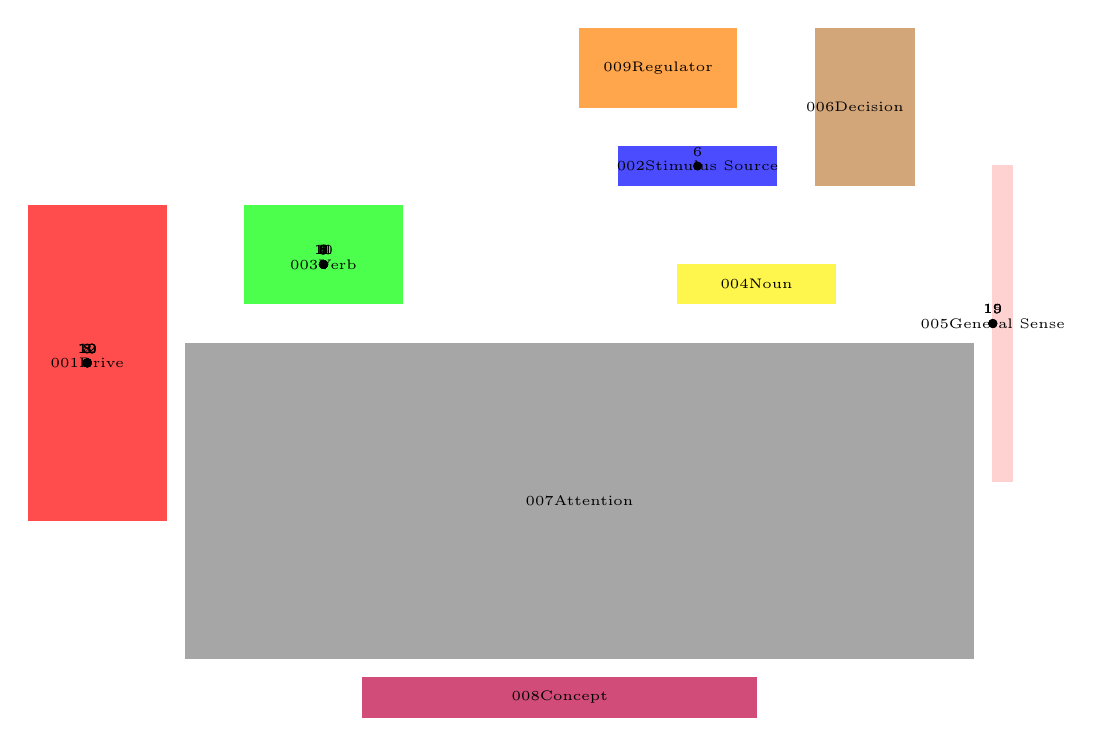
\begin{tikzpicture}[scale=0.25]
\filldraw[red!70] (4,13) rectangle (11,29);
\node at (7,21) {\tiny 001Drive};
\filldraw[blue!70] (34,30) rectangle (42,32);
\node at (38,31) {\tiny 002Stimulus Source};
\filldraw[green!70] (15,24) rectangle (23,29);
\node at (19,26) {\tiny 003Verb};
\filldraw[yellow!70] (37,24) rectangle (45,26);
\node at (41,25) {\tiny 004Noun};
\filldraw[purple!70] (21,3) rectangle (41,5);
\node at (31,4) {\tiny 008Concept};
\filldraw[orange!70] (32,34) rectangle (40,38);
\node at (36,36) {\tiny 009Regulator};
\filldraw[pink!70] (53,15) rectangle (54,31);
\node at (53,23) {\tiny 005General Sense};
\filldraw[brown!70] (44,30) rectangle (49,38);
\node at (46,34) {\tiny 006Decision};
\filldraw[gray!70] (12,6) rectangle (52,22);
\node at (32,14) {\tiny 007Attention};
\filldraw[black] (19,26) circle (0.2);
\node at (19,26) [above, font=\tiny] {1};
\filldraw[black] (19,26) circle (0.2);
\node at (19,26) [above, font=\tiny] {2};
\filldraw[black] (19,26) circle (0.2);
\node at (19,26) [above, font=\tiny] {4};
\filldraw[black] (7,21) circle (0.2);
\node at (7,21) [above, font=\tiny] {10};
\filldraw[black] (7,21) circle (0.2);
\node at (7,21) [above, font=\tiny] {5};
\filldraw[black] (7,21) circle (0.2);
\node at (7,21) [above, font=\tiny] {10};
\filldraw[black] (7,21) circle (0.2);
\node at (7,21) [above, font=\tiny] {10};
\filldraw[black] (7,21) circle (0.2);
\node at (7,21) [above, font=\tiny] {12};
\filldraw[black] (53,23) circle (0.2);
\node at (53,23) [above, font=\tiny] {19};
\filldraw[black] (7,21) circle (0.2);
\node at (7,21) [above, font=\tiny] {12};
\filldraw[black] (53,23) circle (0.2);
\node at (53,23) [above, font=\tiny] {19};
\filldraw[black] (19,26) circle (0.2);
\node at (19,26) [above, font=\tiny] {3};
\filldraw[black] (19,26) circle (0.2);
\node at (19,26) [above, font=\tiny] {5};
\filldraw[black] (19,26) circle (0.2);
\node at (19,26) [above, font=\tiny] {6};
\filldraw[black] (19,26) circle (0.2);
\node at (19,26) [above, font=\tiny] {7};
\filldraw[black] (19,26) circle (0.2);
\node at (19,26) [above, font=\tiny] {8};
\filldraw[black] (19,26) circle (0.2);
\node at (19,26) [above, font=\tiny] {9};
\filldraw[black] (19,26) circle (0.2);
\node at (19,26) [above, font=\tiny] {10};
\filldraw[black] (19,26) circle (0.2);
\node at (19,26) [above, font=\tiny] {11};
\filldraw[black] (7,21) circle (0.2);
\node at (7,21) [above, font=\tiny] {8};
\filldraw[black] (53,23) circle (0.2);
\node at (53,23) [above, font=\tiny] {15};
\filldraw[black] (38,31) circle (0.2);
\node at (38,31) [above, font=\tiny] {6};
\filldraw[black] (7,21) circle (0.2);
\node at (7,21) [above, font=\tiny] {2};
\end{tikzpicture}
\end{center}

\section*{Instincts Legend}

\begin{longtable}{|p{3cm}|p{3cm}|p{3cm}|p{5cm}|}
\hline
{\bf Action} & {\bf Reward/Punish} & {\bf Amount} & {\bf Conditions} \\ \hline
1 & 49 & 255 & Verb (3)[1]~\newline Perception (0)[0]~\newline Perception (0)[0]~\newline  \\ \hline
2 & 49 & 255 & Verb (3)[2]~\newline Perception (0)[0]~\newline Perception (0)[0]~\newline  \\ \hline
4 & 49 & 255 & Verb (3)[4]~\newline Perception (0)[0]~\newline Perception (0)[0]~\newline  \\ \hline
0 & 50 & 255 & Drive (1)[10]~\newline Perception (0)[0]~\newline Perception (0)[0]~\newline  \\ \hline
9 & 49 & 93 & Drive (1)[5]~\newline Perception (0)[0]~\newline Perception (0)[0]~\newline  \\ \hline
1 & 49 & 255 & Drive (1)[10]~\newline Perception (0)[0]~\newline Perception (0)[0]~\newline  \\ \hline
2 & 49 & 255 & Drive (1)[10]~\newline Perception (0)[0]~\newline Perception (0)[0]~\newline  \\ \hline
1 & 49 & 255 & Drive (1)[12]~\newline General Sense (5)[19]~\newline Perception (0)[0]~\newline  \\ \hline
2 & 49 & 112 & Drive (1)[12]~\newline General Sense (5)[19]~\newline Perception (0)[0]~\newline  \\ \hline
3 & 49 & 255 & Verb (3)[3]~\newline Perception (0)[0]~\newline Perception (0)[0]~\newline  \\ \hline
5 & 49 & 255 & Verb (3)[5]~\newline Perception (0)[0]~\newline Perception (0)[0]~\newline  \\ \hline
6 & 49 & 255 & Verb (3)[6]~\newline Perception (0)[0]~\newline Perception (0)[0]~\newline  \\ \hline
7 & 49 & 255 & Verb (3)[7]~\newline Perception (0)[0]~\newline Perception (0)[0]~\newline  \\ \hline
8 & 49 & 255 & Verb (3)[8]~\newline Perception (0)[0]~\newline Perception (0)[0]~\newline  \\ \hline
9 & 49 & 255 & Verb (3)[9]~\newline Perception (0)[0]~\newline Perception (0)[0]~\newline  \\ \hline
10 & 49 & 255 & Verb (3)[10]~\newline Perception (0)[0]~\newline Perception (0)[0]~\newline  \\ \hline
11 & 49 & 255 & Verb (3)[11]~\newline Perception (0)[0]~\newline Perception (0)[0]~\newline  \\ \hline
5 & 49 & 255 & Drive (1)[8]~\newline General Sense (5)[15]~\newline Perception (0)[0]~\newline  \\ \hline
1 & 49 & 255 & Stimulus Source (2)[6]~\newline Drive (1)[2]~\newline Perception (0)[0]~\newline  \\ \hline
\end{longtable}

\section*{Receptors}

\begin{longtable}{|p{2cm}|p{2cm}|p{2cm}|p{2cm}|p{2cm}|}
\hline
{\bf Locus} & {\bf Chemical} & {\bf Threshold} & {\bf Nominal} & {\bf Gain} \\ \hline
(1,5,0) & 1 & 0 & 0 & 255 \\ \hline
(1,5,1) & 2 & 0 & 0 & 255 \\ \hline
(1,5,2) & 3 & 0 & 0 & 255 \\ \hline
(1,5,3) & 4 & 0 & 0 & 255 \\ \hline
(1,5,4) & 5 & 0 & 0 & 255 \\ \hline
(1,5,5) & 6 & 0 & 0 & 255 \\ \hline
(1,5,6) & 7 & 0 & 0 & 255 \\ \hline
(1,5,7) & 8 & 0 & 0 & 255 \\ \hline
(1,5,8) & 9 & 0 & 0 & 255 \\ \hline
(1,5,9) & 10 & 0 & 0 & 255 \\ \hline
(1,5,10) & 11 & 0 & 0 & 255 \\ \hline
(1,5,11) & 12 & 0 & 0 & 255 \\ \hline
(1,5,12) & 13 & 0 & 0 & 255 \\ \hline
(0,6,13) & 49 & 0 & 0 & 255 \\ \hline
(0,6,14) & 50 & 0 & 0 & 255 \\ \hline
(0,8,14) & 52 & 0 & 4 & 255 \\ \hline
(0,6,15) & 53 & 0 & 16 & 255 \\ \hline
(0,6,16) & 70 & 0 & 16 & 255 \\ \hline
(0,8,13) & 51 & 0 & 0 & 255 \\ \hline
(1,2,0) & 63 & 0 & 0 & 255 \\ \hline
(1,2,1) & 13 & 0 & 44 & 255 \\ \hline
(1,4,1) & 66 & 255 & 0 & 255 \\ \hline
(1,2,0) & 64 & 0 & 0 & 255 \\ \hline
(1,0,0) & 56 & 255 & 119 & 255 \\ \hline
(1,0,1) & 56 & 255 & 116 & 255 \\ \hline
(1,0,2) & 56 & 255 & 110 & 255 \\ \hline
(1,0,3) & 56 & 120 & 120 & 255 \\ \hline
(1,0,4) & 56 & 76 & 119 & 255 \\ \hline
(1,0,5) & 56 & 34 & 117 & 255 \\ \hline
(1,3,0) & 59 & 8 & 255 & 255 \\ \hline
(1,4,0) & 17 & 65 & 0 & 255 \\ \hline
(1,4,2) & 255 & 58 & 0 & 255 \\ \hline
(1,4,3) & 255 & 42 & 0 & 255 \\ \hline
(1,4,4) & 4 & 255 & 0 & 255 \\ \hline
(1,4,9) & 1 & 48 & 0 & 255 \\ \hline
(1,4,11) & 10 & 255 & 0 & 255 \\ \hline
(1,4,12) & 12 & 255 & 0 & 255 \\ \hline
(1,4,13) & 7 & 255 & 0 & 255 \\ \hline
(1,4,14) & 6 & 255 & 0 & 255 \\ \hline
(1,4,10) & 59 & 0 & 35 & 255 \\ \hline
(1,4,15) & 68 & 106 & 0 & 255 \\ \hline
(1,4,5) & 7 & 255 & 0 & 255 \\ \hline
(1,4,6) & 59 & 20 & 127 & 255 \\ \hline
\end{longtable}

\section*{Emitters}

\begin{longtable}{|p{2cm}|p{2cm}|p{2cm}|p{2cm}|p{2cm}|}
\hline
{\bf Locus} & {\bf Chemical} & {\bf Threshold} & {\bf Sample Rate} & {\bf Gain} \\ \hline
(0,8,1) & 52 & 0 & 1 & 255 \\ \hline
(0,6,1) & 53 & 0 & 1 & 255 \\ \hline
(0,6,2) & 70 & 0 & 1 & 255 \\ \hline
(1,4,1) & 11 & 0 & 25 & 8 \\ \hline
(1,4,1) & 2 & 0 & 64 & 10 \\ \hline
(1,4,3) & 5 & 0 & 24 & 49 \\ \hline
(1,4,2) & 4 & 0 & 24 & 50 \\ \hline
(1,4,4) & 7 & 0 & 114 & 8 \\ \hline
(1,4,5) & 8 & 0 & 18 & 5 \\ \hline
(1,4,5) & 9 & 0 & 75 & 51 \\ \hline
(1,0,0) & 61 & 0 & 17 & 1 \\ \hline
(1,2,0) & 63 & 0 & 17 & 6 \\ \hline
(1,2,0) & 13 & 0 & 20 & 7 \\ \hline
(1,2,1) & 65 & 0 & 40 & 64 \\ \hline
(1,2,1) & 66 & 0 & 13 & 4 \\ \hline
(1,4,0) & 64 & 0 & 19 & 6 \\ \hline
(1,2,0) & 13 & 0 & 25 & 8 \\ \hline
(1,5,0) & 69 & 255 & 18 & 10 \\ \hline
(1,5,2) & 69 & 255 & 21 & 8 \\ \hline
(1,5,7) & 69 & 255 & 26 & 14 \\ \hline
(1,5,8) & 69 & 255 & 16 & 16 \\ \hline
(1,5,9) & 69 & 255 & 9 & 26 \\ \hline
(1,5,10) & 69 & 255 & 25 & 7 \\ \hline
(1,5,11) & 69 & 255 & 11 & 33 \\ \hline
(1,2,0) & 0 & 0 & 82 & 5 \\ \hline
(1,4,0) & 64 & 0 & 49 & 6 \\ \hline
(1,4,1) & 11 & 0 & 47 & 8 \\ \hline
\end{longtable}

\section*{Stimuli}

\begin{longtable}{|p{2cm}|p{2cm}|p{2cm}|p{2cm}|p{2cm}|p{2cm}|p{2cm}|p{2cm}|}
\hline
{\bf SeqNum} & {\bf Significance} & {\bf SensoryNeu} & {\bf Intensity} & {\bf Locus 1} & {\bf Locus 2} & {\bf Locus 3} & {\bf Locus 4} \\ \hline
1 & 0 & 255 & 0 & (27,16) & (18,16) & (28,16) & (0,0) \\ \hline
2 & 32 & 0 & 255 & (34,64) & (33,16) & (40,16) & (49,16) \\ \hline
3 & 80 & 0 & 255 & (34,48) & (40,16) & (25,16) & (29,8) \\ \hline
4 & 32 & 1 & 255 & (17,75) & (26,32) & (28,16) & (39,16) \\ \hline
5 & 255 & 1 & 255 & (17,80) & (26,32) & (28,16) & (39,16) \\ \hline
6 & 82 & 10 & 255 & (0,0) & (0,0) & (0,0) & (0,0) \\ \hline
7 & 36 & 11 & 255 & (0,0) & (0,0) & (0,0) & (0,0) \\ \hline
8 & 0 & 2 & 255 & (17,25) & (0,0) & (0,0) & (0,0) \\ \hline
9 & 255 & 255 & 0 & (0,0) & (0,0) & (0,0) & (0,0) \\ \hline
10 & 16 & 8 & 255 & (0,0) & (0,0) & (0,0) & (0,0) \\ \hline
11 & 16 & 5 & 255 & (43,32) & (40,16) & (0,0) & (0,0) \\ \hline
12 & 16 & 6 & 255 & (43,16) & (40,16) & (25,16) & (0,0) \\ \hline
13 & 0 & 255 & 0 & (27,8) & (0,0) & (0,0) & (0,0) \\ \hline
14 & 0 & 255 & 0 & (22,3) & (43,16) & (0,0) & (0,0) \\ \hline
15 & 0 & 255 & 0 & (22,3) & (43,16) & (0,0) & (0,0) \\ \hline
16 & 0 & 255 & 0 & (22,2) & (0,0) & (0,0) & (0,0) \\ \hline
17 & 0 & 255 & 0 & (22,2) & (40,8) & (25,8) & (0,0) \\ \hline
18 & 0 & 255 & 0 & (22,3) & (40,16) & (0,0) & (0,0) \\ \hline
19 & 0 & 255 & 0 & (38,50) & (23,16) & (27,16) & (0,0) \\ \hline
20 & 0 & 255 & 0 & (38,66) & (39,77) & (27,16) & (20,16) \\ \hline
21 & 0 & 255 & 0 & (22,8) & (43,16) & (7,16) & (0,0) \\ \hline
22 & 0 & 255 & 0 & (1,255) & (6,255) & (7,112) & (61,32) \\ \hline
23 & 0 & 255 & 0 & (1,32) & (6,8) & (10,8) & (61,16) \\ \hline
24 & 0 & 255 & 0 & (1,32) & (6,8) & (10,8) & (61,16) \\ \hline
25 & 0 & 255 & 0 & (21,16) & (36,32) & (6,16) & (10,16) \\ \hline
26 & 0 & 255 & 0 & (22,22) & (43,16) & (7,32) & (0,0) \\ \hline
\end{longtable}

\section*{Chemical Reactions}

\begin{longtable}{|p{5cm}|p{5cm}|p{2cm}|}
\hline
{\bf Reactants} & {\bf Products} & {\bf Rate} \\ \hline
1*pain++ + 1*none & 1*pain + 1*punishment & 8 \\ \hline
1*need for pleasure++ + 1*none & 1*need for pleasure + 1*punishment & 8 \\ \hline
1*hunger++ + 1*none & 1*hunger + 1*punishment & 8 \\ \hline
1*coldness++ + 1*none & 1*coldness + 1*punishment & 8 \\ \hline
1*hotness++ + 1*none & 1*hotness + 1*punishment & 8 \\ \hline
1*tiredness++ + 1*none & 1*tiredness + 1*punishment & 8 \\ \hline
1*sleepiness++ + 1*none & 1*sleepiness + 1*punishment & 8 \\ \hline
1*loneliness++ + 1*none & 1*loneliness + 1*punishment & 8 \\ \hline
1*crowded++ + 1*none & 1*crowded + 1*punishment & 8 \\ \hline
1*fear++ + 1*none & 1*fear + 1*punishment & 8 \\ \hline
1*boredom++ + 1*none & 1*boredom + 1*punishment & 8 \\ \hline
1*anger++ + 1*none & 1*anger + 1*punishment & 8 \\ \hline
1*sex drive++ + 1*none & 1*sex drive + 1*punishment & 8 \\ \hline
1*pain-- + 1*pain & 1*reward + 1*none & 8 \\ \hline
1*need for pleasure-- + 1*need for pleasure & 1*reward + 1*none & 8 \\ \hline
1*hunger-- + 1*hunger & 1*reward + 1*none & 8 \\ \hline
1*coldness-- + 1*coldness & 1*reward + 1*none & 8 \\ \hline
1*hotness-- + 1*hotness & 1*reward + 1*none & 8 \\ \hline
1*tiredness-- + 1*tiredness & 1*reward + 1*none & 8 \\ \hline
1*sleepiness-- + 1*sleepiness & 1*reward + 1*none & 8 \\ \hline
1*loneliness-- + 1*loneliness & 1*reward + 1*none & 8 \\ \hline
1*crowded-- + 1*crowded & 1*reward + 1*none & 8 \\ \hline
1*fear-- + 1*fear & 1*reward + 1*none & 8 \\ \hline
1*boredom-- + 1*boredom & 1*reward + 1*none & 8 \\ \hline
1*anger-- + 1*anger & 1*reward + 1*none & 8 \\ \hline
1*sex drive-- + 1*sex drive & 1*reward + 1*none & 8 \\ \hline
1*reward + 1*none & 1*reinforcement + 1*rewardecho & 16 \\ \hline
1*punishment + 1*none & 1*reinforcement + 1*punishecho & 16 \\ \hline
1*starch + 1*none & 2*glucose + 1*none & 64 \\ \hline
3*glucose + 1*none & 1*glycogen + 1*hunger-- & 56 \\ \hline
1*glycogen + 1*none & 3*glucose + 1*hunger & 64 \\ \hline
1*glucose + 2*hexokinase & 4*CO2 + 1*none & 24 \\ \hline
1*gonadotropin + 2*estrogen & 1*gonadotropin + 1*none & 40 \\ \hline
1*glycotoxin + 2*glycogen & 2*pain++ + 2*sleepiness++ & 72 \\ \hline
2*antigen 7 + 4*glucose & 1*antigen 7 + 1*hotness & 88 \\ \hline
2*antigen 7 + 4*glucose & 1*antigen 7 + 1*hotness & 88 \\ \hline
2*antigen 7 + 4*glucose & 1*antigen 7 + 1*hotness & 88 \\ \hline
2*antigen 7 + 4*glucose & 1*antigen 7 + 1*hotness & 80 \\ \hline
2*antigen 7 + 4*glucose & 1*antigen 7 + 1*hotness & 80 \\ \hline
2*antigen 7 + 1*glucose & 1*antigen 7 + 1*hotness & 80 \\ \hline
2*antigen 7 + 1*glucose & 1*antigen 7 + 1*hotness & 80 \\ \hline
2*antigen 7 + 1*glucose & 1*antigen 7 + 1*hotness & 80 \\ \hline
4*antigen 7 + 1*none & 2*hotness + 1*hexokinase & 80 \\ \hline
2*antigen 7 + 1*none & 2*sleepiness + 1*tiredness & 64 \\ \hline
1*alcohol + 1*none & 2*anger + 1*sleepiness & 64 \\ \hline
1*alcohol + 1*none & 3*sex drive + 1*sleepiness & 64 \\ \hline
4*adrenaline + 1*glucose & 1*none + 1*none & 96 \\ \hline
1*adrenaline + 1*testosterone & 1*sex drive-- + 1*none & 72 \\ \hline
1*adrenaline + 1*estrogen & 1*sex drive-- + 1*none & 72 \\ \hline
1*adrenaline + 1*none & 1*none + 1*none & 88 \\ \hline
1*hunger-- + 1*hunger & 1*none + 1*none & 32 \\ \hline
1*gonadotropin + 1*glucose & 1*gonadotropin + 1*none & 96 \\ \hline
1*energy + 1*none & 2*glucose + 1*pain++ & 32 \\ \hline
1*adrenaline + 1*none & 2*adrenaline + 1*none & 32 \\ \hline
1*pain killer + 1*none & 2*pain-- + 1*sleepiness++ & 32 \\ \hline
1*cough medicine + 2*antigen 7 & 2*sleepiness++ + 1*none & 32 \\ \hline
1*sleeping pill + 1*none & 2*sleepiness++ + 1*none & 32 \\ \hline
1*wake-up pill + 1*glucose & 2*sleepiness-- + 1*adrenaline & 32 \\ \hline
\end{longtable}

\section*{Chemical Half-Lives}

\begin{longtable}{|p{4cm}|p{4cm}|}
\hline
{\bf Chemical} & {\bf Half-Life} \\ \hline
\end{longtable}

\end{document}
